\documentclass[12pt]{article}
\usepackage{a4wide, amsfonts, epsfig}
 
\begin{document}
\begin{center}
{\bf A Fourier series example\footnote{Conor Houghton, {\tt houghton@maths.tcd.ie},
see also {\tt http://www.maths.tcd.ie/\char126 houghton/MA22S3}}}\\[1cm]{} 17 January 2007, 13 October 2009
\end{center}
The Fourier series for 
\begin{equation}
f(t)=\left\{\begin{array}{ll}-1&-\pi<t<0\\1&0<t<\pi\end{array}\right.
\end{equation}
with $f(t+2\pi)=f(t)$ is
\begin{equation}
f(t)=\frac{4}{\pi}\sum_{n\mbox{ {\scriptsize odd}}}\frac{1}{n}\sin{nt}
\end{equation}
If we write
\begin{equation}
f_N(t)=\frac{4}{\pi}\sum_{n\mbox{ {\scriptsize odd,} }n\le N}\frac{1}{n}\sin{nt}
\end{equation}
then
\begin{center}
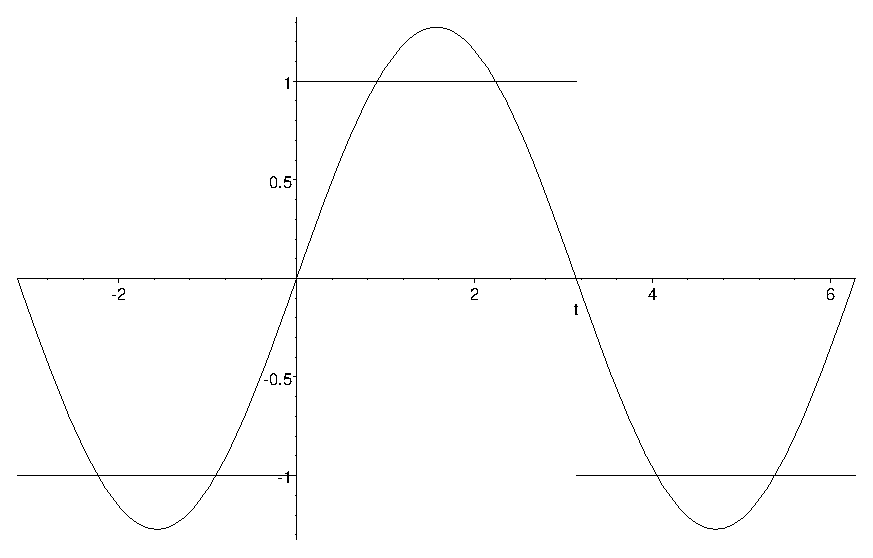
\epsfig{file=1.eps,width=8cm}
$f_1(t)$
\end{center}

\begin{center}
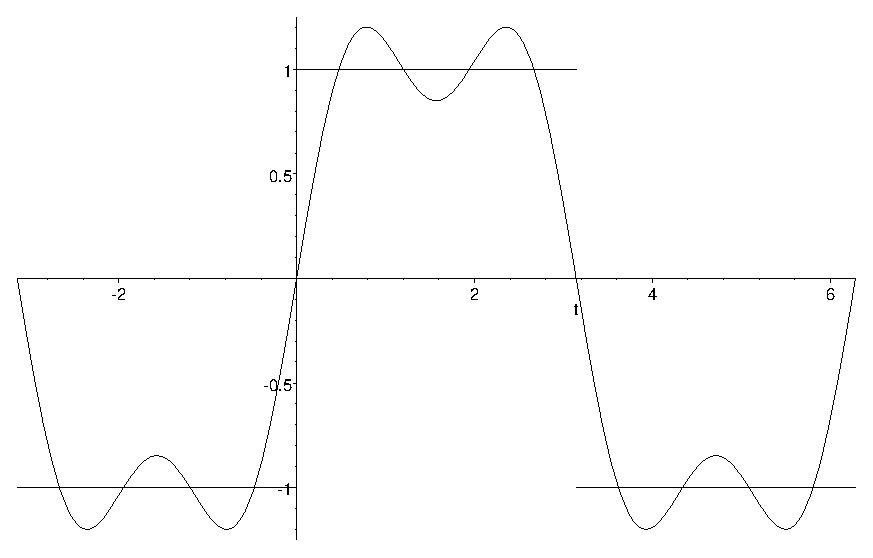
\epsfig{file=3.eps,width=8cm}
$f_3(t)$
\end{center}


\begin{center}
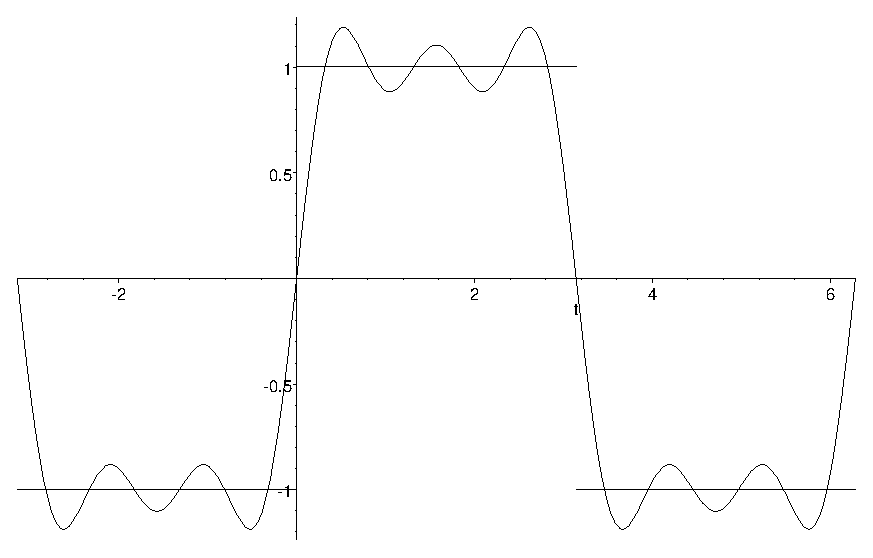
\epsfig{file=5.eps,width=8cm}
$f_5(t)$
\end{center}


\begin{center}
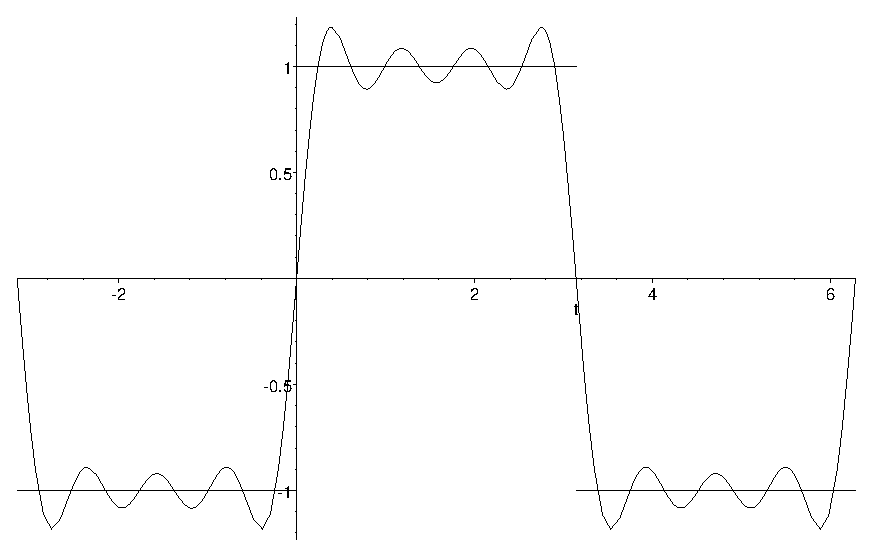
\epsfig{file=7.eps,width=8cm}
$f_7(t)$
\end{center}


\begin{center}
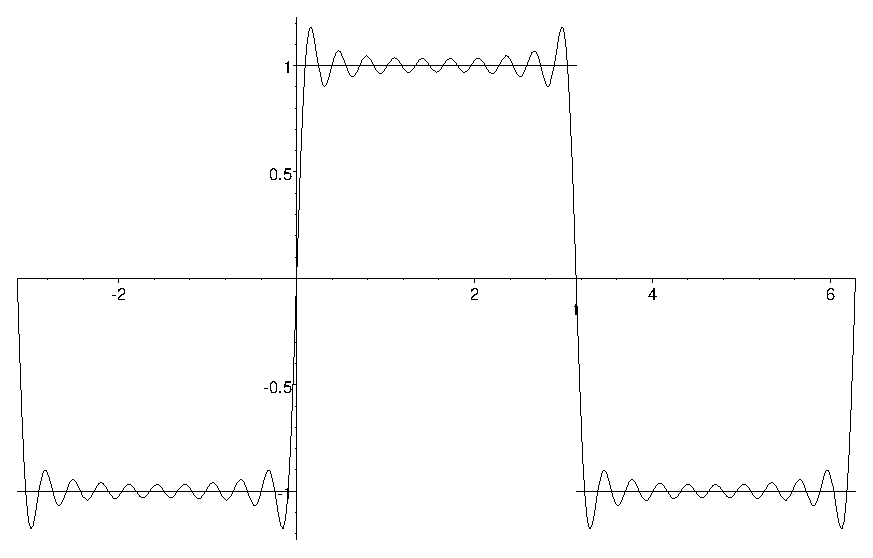
\epsfig{file=19.eps,width=8cm}
$f_{19}(t)$
\end{center}


\end{document}
